\documentclass[]{IEEEtran}

% Your packages go here
\usepackage[utf8]{inputenc}
\usepackage{graphicx}
\usepackage{float}
\usepackage{listings}

\markboth{MC949/MO446 Computer Vision}{}

\begin{document}
  \title{Homework 0}
  \author{Iury Cleveston (RA 230216), Leonardo Rezende (RA 262953) and Thales Oliveira (RA 148051)
    \thanks{iurycl@gmail.com, l262953@dac.unicamp.br, t148051@dac.unicamp.br}
  }

  \maketitle
  
  \begin{abstract}
    In this project the group was able to get in contact with the development environment to be worked with during the Computer Vision Course. The exercises proposed were completed, and the manipulated images are shown throughout this report. By resolving the problems, the group was able to work with OpenCV and related libraries for image manipulation in the Python programming language.
  \end{abstract}
  
  \section{Introduction}
  
  This work, developed by Group 8 of Computer Vision Course (2nd Semester/2019), has the objective of introducing the tools used in the field of Computer Vision, and also to practice programming skills needed to succeed in the following projects. The theme of the exercises is basic image manipulation using OpenCV library, and the group decided to work with the Python programming language. The project consists of 5 exercises, divided by specific parts. The solutions of each question, which can be output images, text answers or both, are listed in the next section (Image outputs and Answers). The Conclusion section sums up the work done. 


  \section{Image outputs and Answers}
  \subsection{Exercise 1}
  For this exercise, it was supposed to find an image to be used as input for the next exercises. The chosen image is displayed in figure \ref{fig:i-1-0}, and it is 300x400 pixels, in order to fit the requirements.
  \begin{figure}[!h]
    \centering
    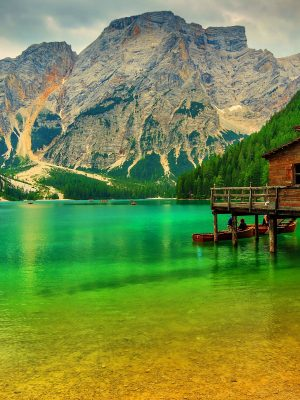
\includegraphics[width=0.8\hsize]{../input/i-1-0.jpg}
    \caption{Image input used for exercises 2 to 5}
    \label{fig:i-1-0}
  \end{figure}
  
  \subsection{Exercise 2}
  
  The first question asked to swap the blue and red channels in the original image. The result can be seen in Figure~\ref{fig:o-2-a-0}.
  
  \begin{figure}[!h]
    \centering
    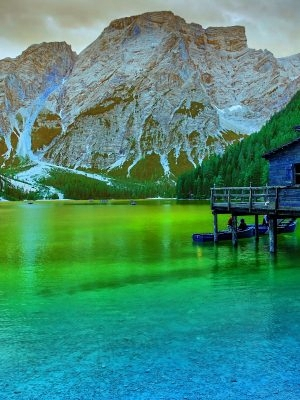
\includegraphics[width=0.8\hsize]{../output/o-2-a-0.jpg}
    \caption{Output image after swapping the blue and red channels.}
    \label{fig:o-2-a-0}
  \end{figure}
  
  In the second question, we should generate a green monochromatic image. This process was executed by selecting the green channel in the original image. The result is presented in Figure~\ref{fig:o-2-b-0}.
  
  \begin{figure}[!h]
    \centering
    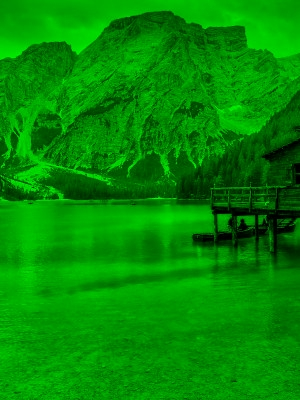
\includegraphics[width=0.8\hsize]{../output/o-2-b-0.jpg}
    \caption{Output image after selecting the green channel.}
    \label{fig:o-2-b-0}
  \end{figure}
  
  In the third question, we should generate a red monochromatic image. This process was executed by selecting the red channel in the original image. The result generated is shown in Figure~\ref{fig:o-2-c-0}.
  
  \begin{figure}[!h]
    \centering
    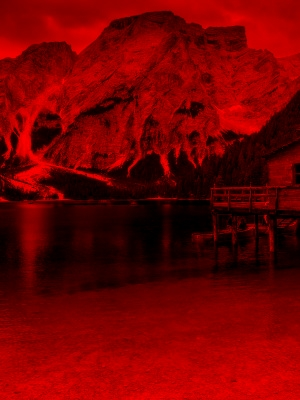
\includegraphics[width=0.8\hsize]{../output/o-2-c-0.jpg}
    \caption{Output image after selecting the red channel.}
    \label{fig:o-2-c-0}
  \end{figure}
  
  The green monochrome image looks better because it holds more information than the red one, which has many areas in dark. The computer vision algorithm should perform better in the green image because the saliency map can be identified easily and the feature description can be more useful.
  
  \subsection{Exercise 3}
  For this exercise, the green monochrome image from previous exercise (labed here image A), is manipulated with the red monochrome image from the same problem (labed here as B). The figure \ref{fig:o-3-0} represents image B, with the 100x100 central pixels from image A.  
  \begin{figure}[!h]
    \centering
    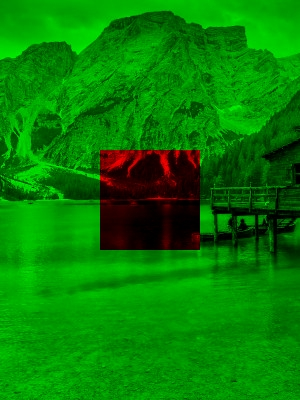
\includegraphics{../output/o-3-0.jpg}
    \caption{Image B manipulated with image A specific region}
    \label{fig:o-3-0}
  \end{figure}
  Next, the red channel from image B (modified) is replaced in the original image. The figure \ref{fig:o-3-1} represents this operation. Inspecting the figure, we can see that in the 100x100 central pixels of the image, there is no presence of the red color, as the red channel has zero values in that region, creating a "greenish" appearance for those pixels. 
  
  \begin{figure}[!h]
    \centering
    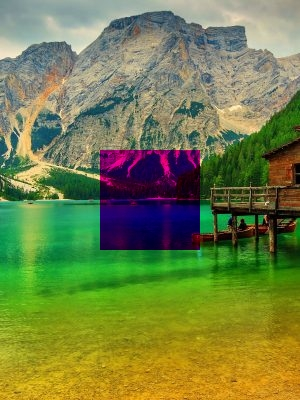
\includegraphics{../output/o-3-1.jpg}
    \caption{Original image with red channel from image B}
    \label{fig:o-3-1}
  \end{figure}

\subsection{Excercise 4}
  Here we aply some arithmetic and geometric operations to green monochrome to extract some important values and see what they can change at the image.
  These values are:
  \begin{itemize}
    \item{Max value: 238}
    \item{Min value: 0}
    \item{Mean value: 138.79}
    \item{Standard deviation: 38.07}
  \end{itemize}


  To extract mean and standard values, we used this opencv function:
  \begin{lstlisting}     
    green_channel = image[:,:,1]
    mean, stdev = cv2.meanStdDev(green_channel)
  \end{lstlisting}  

  Then, we used mean and standard deviation to normalize the values, as suggested on the answer and implemented in the following code:
  \begin{lstlisting}     
    green_channel = ((green_channel - mean)/stdev*10).astype(int)
    image[:,:,1] = image[:,:,1] + green_channel    
  \end{lstlisting}  
  We can see the result on Figure \ref{fig:o-4-b-0}. Seems like the image got a beter contrast, as the values got normalized. The higher-value pixels got more bright (255), and the lower-value got more dark (0).
  \begin{figure}[!h]
    \centering
    \includegraphics[width=0.8\hsize]{../output/o-4-b-0.jpg}
    \caption{Output image after normalization.}
    \label{fig:o-4-b-0}
  \end{figure}

  Then, we shifted the image two pixels to the left, using a mask and opencv's warpAffine. The result can be seen at Figure \ref{fig:0-4-c-0}. After that, we took the original green monochrome and substracted Figure \ref{fig:0-4-c-0} from it, leading to Figure \ref{fig:0-4-c-1}. Pixels near to each other that had close values between them resulted in a very low value (sometimes negative). By the other hand, when the values was too different and the shifted one was darker than the original, the resulting pixel was bright. That indicates the borthers on the image, espacially those left-to-right. 

  \begin{figure}[!h]
    \centering
    \includegraphics[width=0.8\hsize]{../output/o-4-c-0.jpg}
    \caption{Output image after normalization.}
    \label{fig:0-4-c-0}
  \end{figure}

  \begin{figure}[!h]
    \centering
    \includegraphics[width=0.8\hsize]{../output/o-4-c-1.jpg}
    \caption{Output image after normalization.}
    \label{fig:0-4-c-1}
  \end{figure}


  \subsection{Exercise 5}
  
  In this exercise, we should take the original colored image and add gaussian noise to the pixels in the green channel. The sigma was defined as 20. The noise increase as the sigma increased. The image seems corrupted as shown in Figure~\ref{fig:o-5-a-0}.
  
  \begin{figure}[!h]
    \centering
    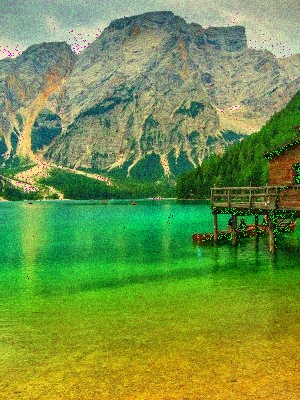
\includegraphics[width=0.8\hsize]{../output/o-5-a-0.jpg}
    \caption{Output image after adding noise to the green channel.}
    \label{fig:o-5-a-0}
  \end{figure}
  
  In the second question, we should the the same gaussian noise the blue channel. The result is shown in Figure~\ref{fig:o-5-b-0}.
  
   \begin{figure}[!h]
    \centering
    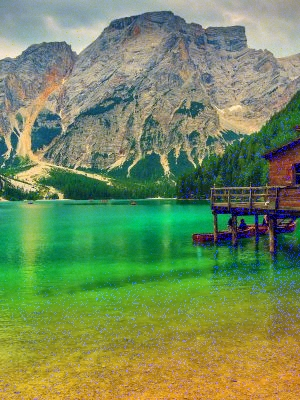
\includegraphics[width=0.8\hsize]{../output/o-5-b-0.jpg}
    \caption{Output image after adding noise to the blue channel.}
    \label{fig:o-5-b-0}
  \end{figure}
  
  The image in which the blue channel received the noise looks better because the blue channel holds less information in terms of saliency and high energy regions than the other channels. So the added noise produced a little impact on the image's content.
  
  
  \section{Conclusion}
  
  In this work, the group dealt with questions related to basic image manipulation, in order to get used to the development environment of the course. The team was able to complete all exercises proposed, and the generated output is present in this report.

\end{document}
